\chapter{Opis rozwiązania}
\label{cha:Opis rozwiązania}

W poniższym rozdziale omówione zostaną kroki pracy.

\section{Transmisja danych}
\label{sec:transmisjaDanych}

Pierwszym aspektem który należy rozwiązać jest sposób przesyłania danych. Problem ten jest szczególnie istotny w omawianej pracy z uwagi na możliwość przesyłania dużej ilości informacji o granicach lub innych liniach przezentowanych na mapie. Do opisu kwadratowego obszaru wymagane jest przesłanie informacji o minimum 4 punktach. Jeżeli będziemy chcieli przekazać dokłądniejszy zarys obszaru, zaprezentować granicę państwa lub linię frotnu wojennego linia prosta w większości przypadków będzie zbyt ogólnym przybliżeniem, nie oddającym prawdziwej sytuacji.

Projekt zakłada korzystanie z lokalnej pamięci komputera użytkownika podczas pracy, jednak dostarczenie informacji, danych wejściowych nie powinno być ograniczone do wczytania ich z pliku tekstowego, należy pamiętać o możliwości przesłania ich z serwera aplikacji do użytkownika. W sytuacji takiej, gdzie w jednym momencie przesłane zostaja wszystkie informacje na któch będzie zachodzia praca, ilość informacji może być znaczna.

Z raportu Akamai wynika że śrenia przepływność łączy internetowych dla użytkowników korzystających z puli adresów IP przeznaczonych dla Polski w I kwartale 2012 r. wynosiła 5Mb/s  \underline{\texttt{http://www.rp.pl/artykul/924483.html}} (dostęp 13.04.2014). Jest to bardzo dobry wynik który plasuje Polskę w czołówce rankingu. Pomimo tego nie można pominąć faktu optymalizacji zapytać i danych przesyłanych, wymieniane dane pomiędzy użytkownikiem a serwerem powinny być jak najmniejsze. Duża popularność urządzeń mobilnych w których dostęp do internetu jest zapewniany często poprzez sieć bezprzewodową a dostęp do interentu nie jest jeszcze tak dogodny jak jest to w przypadku użytkowników stacjonarnych  wymusza optymalizację.

Kolejnym powodem dla którego odpowiedzi serwera powinny być jak najlżesze jest koszt pracy samego serwera. Jest to szczególnie widoczne w dużych aplikacjach mających wiele urzytkowników, czas jaki jest przeznaczany dla pojedyńczego użytkownika jest mnożony przez ich ilość. Z tego powodu zawsze podczas zwiększania ilości użtkowników korzystających z aplikacji następuje czas w którym należy zacząć korzystać z dodatkowego serwera. Celem programisty tworzącego kod który będzie wykorzystywał zasoby serwera(zarówno czas jak i pamięć) jest dbanie aby moment w którym niezbędne będzie korzystanie z większej ilośći maszym nastąpił przy jak największej ilości użytkowników.

xml - 729  557
json - 695  400




\subsection{Format zapisu}
\label{subsec:zapis}

Istnieje wiele formatów używanyc w zależności od konkretnych potrzeb. Można dokonać ogólnego podziału na dwa rodzaje. Pierwszym są pliki zapisane rastrowo, jest to zapis punktów o określonym kolorze i położeniu na płaszczyźnie. Efektem takiego podejścia jest pogorszenie obrazu w momencie dużego powiększenia. Przykładem są formaty takie jak ADRG,ASC czy RGB.
Porównanie litery a i jej 7-krotnego powiększenia w tym zapise zaprezentowano na rysunku \ref{fig:rast}
  \begin{figure}[H]
  \centering
    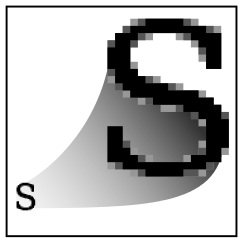
\includegraphics[width=50mm]{ge/a2.jpg}
  \caption{Zapis rastrowy}
  \label{fig:rast}
  \end{figure}

Innym podejściem jest zapis wektorowy. Jest to zapis oparty na formułach matematycznych m.in. proste i łuki. Dzięki takiemu podejściu obraz w dowolnej skali na identyczną jakość, widać to na rysunku \ref{fig:wekt}. Przykładowymi formatami są GML(Geography Markup Language) otwarty standart XML dla wymiany danych GIS,Shapefile czy tradycyjny kartezjański układ współrzędnych.

  \begin{figure}[H]
  \centering
    
\includegraphics[width=50mm]{ge/a1.jpg}
  \caption{Zapis wektorowy}
  \label{fig:wekt}
  \end{figure}

Do celów projektu zdecydowano się skorzystać z zapisu wektorowego. Oprócz bez problemowej skalowalności, pozwala on również na szeroką i łatwą edycję. W prosty sposób można dodać informacje nie tylko o położeniu, ale inne takie jak słowny opis miejsca lub wydarzenia które miało miejsce w pobliskim rejonie.

Format KML jest używany do reprezentacji danych graficznych w aplikacjach firmy Google, takich jak Google Maps czy Google Earth. Oparty jest na standardzie XML, wrażliwy na wielkość liter, wymusza ścisłą poprawność danych z formatem. Oznacza to że każdy tag, element ma ścisle określone miejsce i nie może pojawić się nigdzie indziej.

Aby tworzona aplikacja miała możliwość współpracy ze stworzonymi wczesniej zbiorami danych, mapami mimo faktu iż informacje te nie będą w pełni wykorzystywały możliwości frameworku, stworzony został parser plików kml. Dzięki temu możliwy jest import danych, uzupełnienie ich o dodatkowe informacje i zapis do własnego formatu.

\section{Parser plików}
\label{sec:parser}

Założenia projektu zapewniają dwa źródła dostarczania informacji niezbędnych do poprawnej pracy frameworka.
Pierwszym jest przesyłanie infromacji z serwera do urządzenia klienta przy wykorzystaniu formatu JSON, wiadomość taka jest zbudowana w odpowiednią strukturę aby bezpośrednio dokonać konwersji do jegnego ciągu znakowego. W ten sposób możliwe będzie zapewnienie w bardzo szybkim czasie danych pozwalających na pełne wykorzystanie wszystkich możliwości aplikacji.

Dodatkową opcją dostarczania informacji będzie wczytywanie pliku z informacjami opisującymi mapę. Do tego celu stworzono parser plików który pozwala na dokonanie analizy wczytanego pliku i konwersję danych do formatu używanego do przechowywania danych po stronie klienta.

\section{Oś czasu}
\label{sec:timeLine}

Tematem pracy oprócz wykorzystania i prezentacji danych na bazie informacji geograficznych jest ich połączenie z osią czasu, która pozwoliłaby na zmianę prezentowanych danych ze względu na interesujący nas okres czasu.

Ponieważ własna implementacja osi czasu która nieograniczałaby użytkownika, pozwala mu w pełni korzystać z możliwości pełnej aplikacji, która tylko w części składa się z możliwości manipulacji czasem postanowiono wykorzystać istniejące rozwiązanie.

Przeprowadzając badania rozwiązań głównymi aspektami na które zwrócono uwagę było:

\begin{itemize}

\item

Typ licencji
Niezwykle ważne jest aby końcowy projekt był całkowicie otwarty dla dalszego rozwoju, pozwalał użytkownikom na adaptację rozwiązań dla swoich potrzeb. Z uwagi na to licencja musi pozwalać na nieograniczoną modyfikację kodu źródłowego.

\item

Wykorzystywane technologie
Pamiętając że efektem końcowym powinien być framework odpowiadający szerokiemu gronowi odbiorców, będący jednocześnie darmowym ważne aby języki programowania wykorzystane przy jego tworzeniu też taki były. Oznacza to nie korzystanie z płatnych, wymagających licencji oprogramowań. Używane standarty powinny być rozpropagowane i używane przez szerokie grono obiorców.

\end{itemize}

Po długich i wnikliwych poszukiwaniach zdecydowano skorzystać z widget-u o nazwie Timeline który został stworzony przej projekt SIMILE działający na uczelni MIT. Pozwala on na bardzo dużą konfigurowalność dzięki czemu jego modyfikacja, nawet bez ingerencji w kod źródłowy jest bardzo prosta.
Projekt jest w stanie stworzyć kilka pasm któe będą określały interwały czasu. Pozwala to aby wynik końcowy był przejżysty bez względu czy prezentujemy wydarzenia które miały miejsce w okresie kilku minut czy setek lat.

Problemem który pojawił się było połączenie wybranego sposobu prezentacji osi czasu z mapą i elementami które powinny zmieniać się wraz z upływem czasu.

Rysunek \ref{fig:tm1} prezentuje możliwości tego projektu. Pasmo odpowiadają zakresom czasu, nie muszą on jednak być jednakowe w każdym miejscu. W zaprezentowanym przykładie dzień 23 listpoada uznany został za warty dokładniejszemu przyjżeniu,łatwo możemy z dokładnością co do godziny zmieniać zakres czasu.Natomiast kolejny miesiąc może być o wiele mniej ciekawy, a obszar przeznaczony dla niego być mniejszy niż ten posiadany przez wymieniony powyżej dzień.

Dla porównania \ref{fig:tm2} prezentuje o wiele prostszą konfigurację w której dolne pasmo podzielone jest przez miesiące, natomiast góre przez tygodnie.

  \begin{figure}[H]
  \centering
    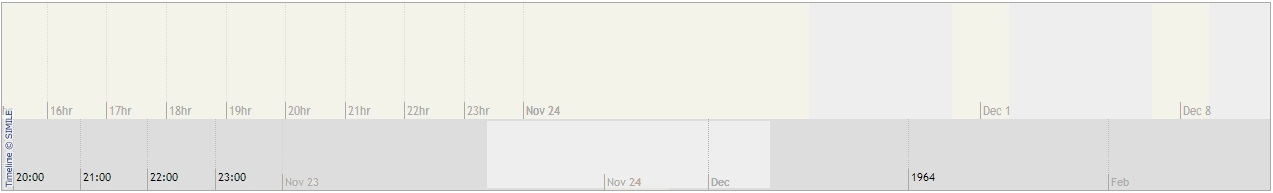
\includegraphics[width=150mm]{ge/tm1.jpg}
  \caption{Timeline}
  \label{fig:tm1}
\end{figure}

  \begin{figure}[H]
  \centering
    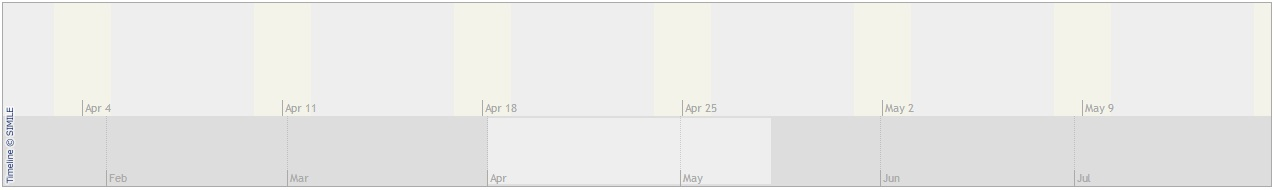
\includegraphics[width=150mm]{ge/tm2.jpg}
  \caption{Timeline 2}
  \label{fig:tm2}
\end{figure}

\section{Interferjs}
\label{sec:Interferjs}

Aby tworzone rozwiązanie mogło być używane przez szerokie grono odbiorców niezbędnym elementem jest stworznie interfejsu który pozwlałby na edycję danych wczytanych z pliku, lecz także pozwalał na stworzenie nowej mapy. W tym celu stworzono interfejs graficzny do edycji danych.
